\section{Source Code and Artifacts}\label{sec:appendix-source-code}

This appendix lists the main source-code files, workflow exports, evaluation files, and supporting evidence used in the thesis. The full project repository is available at:

\begin{quote}
\url{https://github.com/Rumple12/new-yacoub-thesis}
\end{quote}

The appendix does not reproduce source code in full. Instead, it points to the repository artifacts needed to inspect, repeat, or extend the work.

\subsection{Implementation Files}\label{subsec:appendix-implementation-files}

The main implementation files are listed below.

\begin{table}[H]
  \centering
  \small
  \renewcommand{\arraystretch}{1.15}
  \caption{Main implementation artifacts.}
  \label{tab:appendix-implementation-artifacts}
  \begin{tabularx}{\textwidth}{@{}L{0.42\textwidth}Y@{}}
    \toprule
    Path & Purpose \\
    \midrule
    \path{infrastructure/docker/docker-compose.yml} & Docker Compose setup for the local n8n runtime. \\
    \path{middleware/api/routes.py} & Python middleware HTTP routes for status and simulated fan actions. \\
    \path{middleware/gpio/mock_sensor.py} & Simulated sensor and fan-state logic. \\
    \path{scripts/collect_metrics.py} & Script used to collect workflow result rows. \\
    \path{scripts/aggregate_results.py} & Script used to regenerate processed result summaries. \\
    \bottomrule
  \end{tabularx}
\end{table}

\subsection{Workflow, Prompt, and Contract Artifacts}\label{subsec:appendix-workflow-contract-artifacts}

The workflow exports, prompt files, and shared contracts are listed below.

\begin{table}[H]
  \centering
  \small
  \renewcommand{\arraystretch}{1.15}
  \caption{Workflow, prompt, and contract artifacts.}
  \label{tab:appendix-workflow-contract-artifacts}
  \begin{tabularx}{\textwidth}{@{}L{0.42\textwidth}Y@{}}
    \toprule
    Path & Purpose \\
    \midrule
    \path{cognitive_logic/workflows/deterministic-baseline.json} & Exported deterministic baseline n8n workflow. \\
    \path{cognitive_logic/workflows/deterministic-baseline.md} & Description of the deterministic workflow. \\
    \path{cognitive_logic/workflows/agent-minimal.json} & Exported agent-enhanced n8n workflow. \\
    \path{cognitive_logic/workflows/agent-minimal.md} & Description of the agent-enhanced workflow. \\
    \path{cognitive_logic/prompts/system-prompt-v1.md} & Prompt used by the agent-enhanced workflow. \\
    \path{cognitive_logic/memory/memory-choice-v1.md} & Documented memory choice for the agent-enhanced workflow. \\
    \path{shared_interfaces/json-schema/sensor-event.schema.json} & JSON schema for sensor-style temperature events. \\
    \path{shared_interfaces/json-schema/agent-action.schema.json} & JSON schema for contract-shaped action output. \\
    \path{shared_interfaces/examples/} & Example sensor and action payloads. \\
    \bottomrule
  \end{tabularx}
\end{table}

\subsection{Safety and Validation Artifacts}\label{subsec:appendix-safety-validation-artifacts}

The validation and safety-layer documents are listed below. These files define the documented validation cases used in the report.

\begin{table}[H]
  \centering
  \small
  \renewcommand{\arraystretch}{1.15}
  \caption{Safety and validation artifacts.}
  \label{tab:appendix-safety-validation-artifacts}
  \begin{tabularx}{\textwidth}{@{}L{0.42\textwidth}Y@{}}
    \toprule
    Path & Purpose \\
    \midrule
    \path{safety_layer/policies/action-policy-v1.md} & Action policy for allowed and unsupported action outputs. \\
    \path{safety_layer/parsers/output-validation-v1.md} & Documented parser and validation design. \\
    \path{safety_layer/approvals/hitl-v1.md} & Human-in-the-loop approval design. \\
    \path{safety_layer/examples/} & Allowed, blocked, and risky validation examples. \\
    \path{evaluation/datasets/test-cases.json} & Defined workflow and safety test cases. \\
    \bottomrule
  \end{tabularx}
\end{table}

\subsection{Evaluation Result Files}\label{subsec:appendix-evaluation-artifacts}

The main raw and processed result files used in the report are listed below.

\begin{table}[H]
  \centering
  \small
  \renewcommand{\arraystretch}{1.15}
  \caption{Evaluation result artifacts.}
  \label{tab:appendix-evaluation-artifacts}
  \begin{tabularx}{\textwidth}{@{}L{0.42\textwidth}Y@{}}
    \toprule
    Path & Purpose \\
    \midrule
    \path{evaluation/results/raw/run_20260429T165733Z_deterministic.csv} & Final deterministic workflow result rows. \\
    \path{evaluation/results/raw/run_20260429T165859Z_agent.csv} & Final agent-enhanced workflow result rows. \\
    \path{evaluation/results/raw/dump/run_20260429T165702Z_deterministic.csv} & Non-final setup evidence from an earlier HTTP 404 webhook attempt. \\
    \path{evaluation/results/processed/summary_latency.csv} & Processed latency summary. \\
    \path{evaluation/results/processed/summary_resources.csv} & Processed resource summary. \\
    \path{evaluation/results/processed/baseline_vs_agent.csv} & Processed deterministic-versus-agent summary. \\
    \path{evaluation/results/processed/safety_outcomes.csv} & Safety outcome summary file; header only in the final evidence. \\
    \path{evaluation/results/pi-validation/pi-workflow-run-final.csv} & Raspberry Pi middleware/action-endpoint validation rows. \\
    \path{evaluation/results/pi-validation/pi-validation-notes.md} & Raspberry Pi validation notes. \\
    \bottomrule
  \end{tabularx}
\end{table}

\subsection{Figure and Screenshot Evidence}\label{subsec:appendix-figure-screenshot-evidence}

The main report uses selected diagrams and screenshots. Additional raw screenshots and supporting evidence are kept in the repository instead of being reproduced throughout the report.

\begin{table}[H]
  \centering
  \small
  \renewcommand{\arraystretch}{1.15}
  \caption{Figure and screenshot evidence locations.}
  \label{tab:appendix-figure-screenshot-evidence}
  \begin{tabularx}{\textwidth}{@{}L{0.42\textwidth}Y@{}}
    \toprule
    Path & Purpose \\
    \midrule
    \path{thesis/MiunThesisTemplate-master/MiunThesisTemplate-master/Figures/} & Figures and screenshots included in the thesis. \\
    \path{docs/architecture/} & Mermaid sources and notes for architecture and theory diagrams. \\
    \path{cognitive_logic/workflows/evidence/step-06/} & Deterministic workflow screenshot evidence. \\
    \path{cognitive_logic/workflows/evidence/step-07/} & Agent-enhanced workflow screenshot evidence. \\
    \path{evaluation/results/pi-validation/} & Raspberry Pi validation screenshots, notes, and CSV evidence. \\
    \bottomrule
  \end{tabularx}
\end{table}

Figure~\ref{fig:appendix-n8n-runtime-proof} shows one example of local runtime evidence. Other raw screenshots are listed by folder above rather than inserted individually.

\begin{figure}[H]
    \centering
    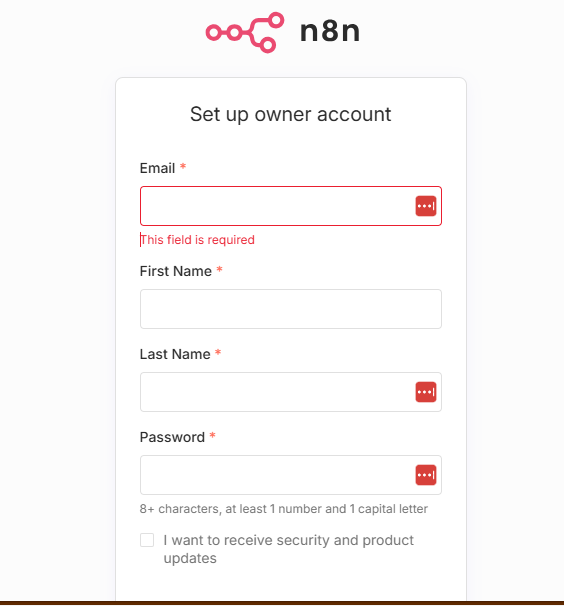
\includegraphics[width=0.55\textwidth]{Figures/n8n-localhost-5678-success-2026-04-25.png}
    \caption{Local n8n runtime verification at localhost port 5678.}
    \label{fig:appendix-n8n-runtime-proof}
\end{figure}

Figure~\ref{fig:appendix-detailed-final-architecture} shows the detailed architecture diagram kept as supporting evidence.

\begin{figure}[H]
    \centering
    \makebox[\textwidth][c]{%
        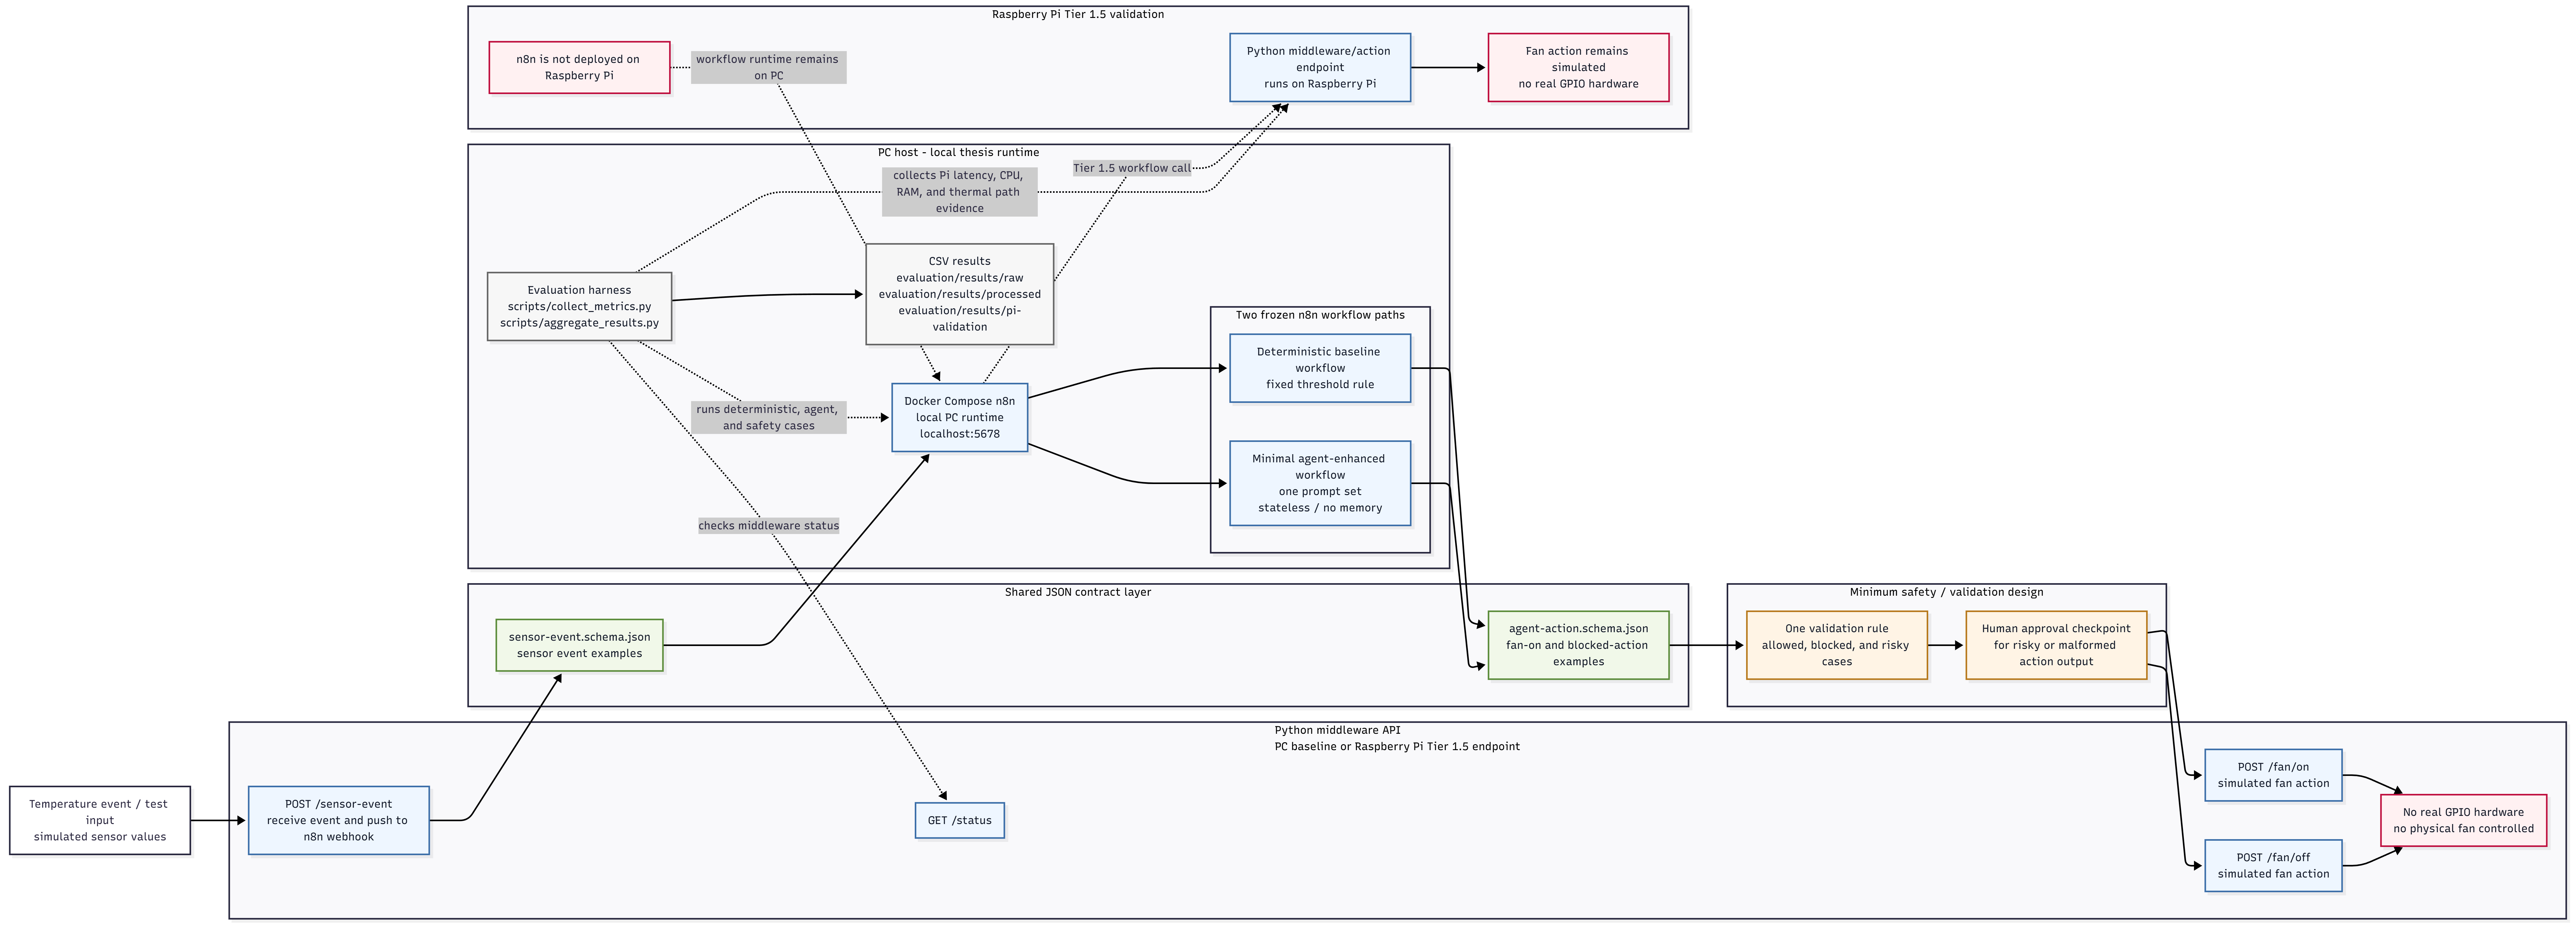
\includegraphics[width=1.08\textwidth]{Figures/appendix-detailed-final-architecture.png}%
    }
    \caption{Detailed architecture diagram preserved as supporting evidence.}
    \label{fig:appendix-detailed-final-architecture}
\end{figure}

Figure~\ref{fig:appendix-pi-middleware-cpu-ram} shows the Raspberry Pi middleware CPU and RAM observation used as supporting resource evidence.

\begin{figure}[H]
    \centering
    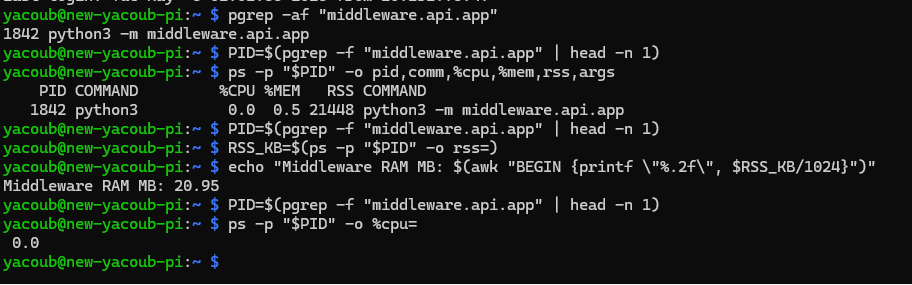
\includegraphics[width=0.95\textwidth]{Figures/appendix-pi-middleware-cpu-ram.png}
    \caption{Raspberry Pi middleware CPU and RAM observation.}
    \label{fig:appendix-pi-middleware-cpu-ram}
\end{figure}

Figures~\ref{fig:appendix-pi-terminal-high-temp-fan-on} and~\ref{fig:appendix-pi-terminal-low-temp-fan-off} show terminal evidence for the Raspberry Pi high- and low-temperature validation cases.

\begin{figure}[H]
    \centering
    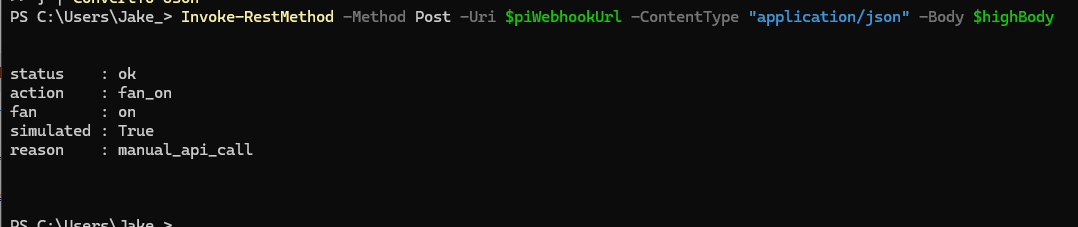
\includegraphics[width=0.95\textwidth]{Figures/appendix-pi-terminal-high-temp-fan-on.png}
    \caption{Raspberry Pi terminal evidence for the high-temperature fan-on case.}
    \label{fig:appendix-pi-terminal-high-temp-fan-on}
\end{figure}

\begin{figure}[H]
    \centering
    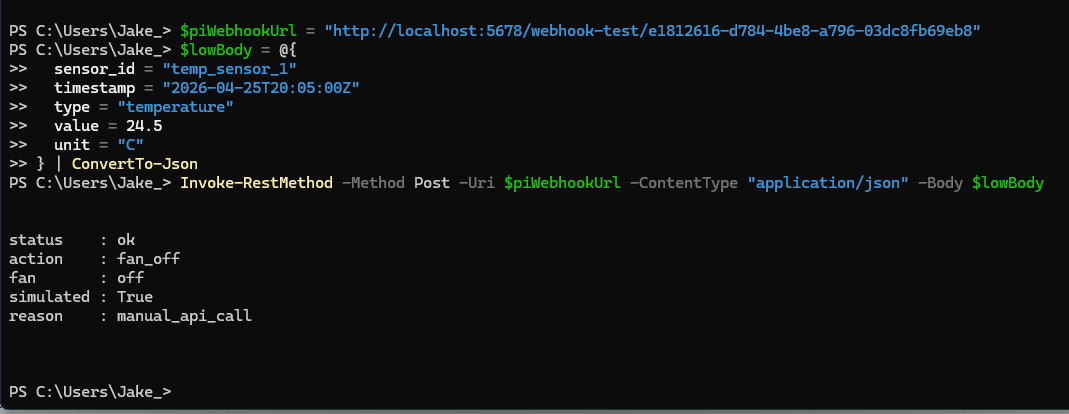
\includegraphics[width=0.95\textwidth]{Figures/appendix-pi-terminal-low-temp-fan-off.png}
    \caption{Raspberry Pi terminal evidence for the low-temperature fan-off case.}
    \label{fig:appendix-pi-terminal-low-temp-fan-off}
\end{figure}
